%************************************************
\chapter{Auswertung}\label{ch:end} 
%************************************************

Die vorangegangenen Kapitel zeigen, dass die Migration einer komplexen Software keineswegs trivial ist. Gleichzeitig vereinfachen verschiedene Technologien die 
sowohl die Arbeit, als auch die Beachtung des Standards \textbf{ISO/IEC 14764}. Die Anforderungsanalyse in Kapitel~\ref{analyze} zeigt, dass eine manuelle Erkennung 
des zu ändernden Codes aufgrund der Menge nahezu unmöglich ist und nur mit technischen Hilfsmitteln wie dem in Kapitel~\ref{automatic} vorgestellten \textit{php7mar} 
zu überblicken ist. Dazu ist jedoch auch zu erwähnen, dass diese Hilfsmittel unter Umständen fehlerhaft sind oder nicht alle Bereiche der Migration abdecken und 
dementsprechend erst (weiter-) entwickelt werden müssen. Die in \textbf{ISO/IEC 14764} geforderte Unterstützung des historischen Codes kann zwar auf klassischem Wege 
gelöst werden, stellt sich jedoch, wie in Kapitel~\ref{VCS} dargelegt, für umfangreiche Projekte nur unter Verwendung von Virtualisierung als sinnvoll dar. 
Die in Kapitel~\ref{develop} gezeigten Änderungen an der Software zeigen, wie wichtig die aufgezeigten Techniken des Refactorings für die Migration einer Software sind.
Zudem zeigen diese Änderungen, dass zwei der in Kapitel~\ref{ch:php7} herausgearbeiteteten Ziele des neuen Major-Release von \ac{PHP} erreicht wurden: \\
So zeigen beispielsweise die Kapitel~\ref{indirect} und \ref{construct}, dass Sonderfälle reduziert wurden und Sprachkonstrukte in \ac{PHP} vereinheitlicht wurden. 
Das Ziel der erhöhten Sicherheit von Software wird über die Entfernung veralteter Erweiterungen (vgl. Kapitel~\ref{mysql}) sowie potentiell gefährlicher Optionen (vgl. Kapitel~\ref{preg}) 
erreicht. Das letzte Ziel, die Erhöhung der Ausführungsgeschwindigkeit, lässt sich über das in Kapitel~\ref{newrelic} vorgestellte Tool \textit{New Relic} überprüfen. 
Eine Auswertung der 24 Stunden vor, sowie nach der Migration (dargstellt in Abbildung~\ref{fig:time}) zeigt, dass die durchschnittliche Ausführungszeit von Anfragen an den Onlineshop 
von 66,05ms auf 43,38ms und somit um ca. 34\% zurückgegangen ist.

\begin{figure}[bth]
    \myfloatalign
    {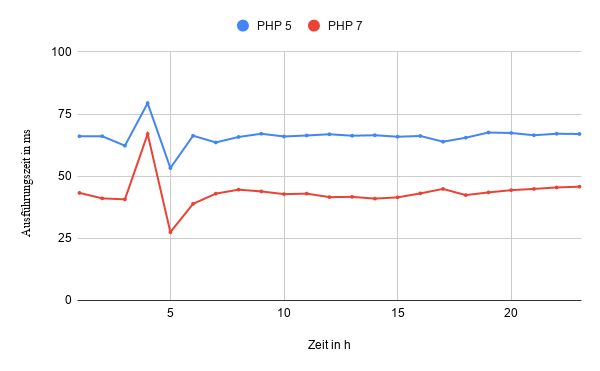
\includegraphics[width=1\linewidth]{gfx/chart}} \quad
    \caption[Ausführungszeiten von Anfragen vor und nach der Migration]{Ausführungszeiten von Anfragen vor und nach der Migration}\label{fig:time}
\end{figure}


\chapter{Schlussbetrachtungen}
Die gezeigte Migration eines großen Softwareprojekts ist, gerade angesichts der schon angekündigten achten Version von \acs{PHP}, 
bei weitem keine einzigartige Aufgabe in der Softwareentwicklung. Trotz des großen Aufwandes scheint es keine Bestrebungen 
zu geben, diese Aufgabe umfänglich zu automatisieren. Daraus ergibt sich die Möglichkeit, in einer weiteren Arbeit die 
Möglichkeiten hinsichtlich einer Automation einer Softwaremigration zu evaluieren. Ein möglicher Ansatz ist die Dokumentation 
von Änderungen in einer geeigneten Beschreibungssprache. Weitere mögliche Betrachtungen des Themas ergeben sich hinsichtlich 
der Codequalität eines Softwareprojekts und den Auswirkungen dieser auf eine Migration. Erste Ansichten dazu finden sich in \cite{martin_clean_2012}.

\subsection{Danksagung}
Hiermit bedanke ich mich bei Allen, die mich bei der Fertigstellung dieser Arbeit unterstützt haben. 
Ein herzlicher Dank gebührt ebenso Jonas Stahl und dem gesamten Team der Firma \textit{tickets75} für die gleichsam wertvolle 
und nette Zusammenarbeit und die tolle Unterstützung.
 
